\documentclass[a4paper,twoside,12pt]{report}

\usepackage{amsmath}
\usepackage{amssymb}
\usepackage{amsthm}
\usepackage[labelfont=bf,labelsep=period]{caption}
\usepackage{enumitem}
\usepackage{float}
\usepackage[margin=2.5cm]{geometry}
\usepackage{graphicx}
\graphicspath{ {./images/} }
\usepackage{numbertabbing}
\usepackage{times}
\usepackage{url}
\usepackage{xspace}
\usepackage{hyperref}

\floatstyle{ruled}
\newfloat{algo}{htbp}{algo}
\floatname{algo}{Algorithm}

%%% fill in your data here %%%
\newcommand{\thesistitle}{A concurrent DEX on Cardano}
\newcommand{\thesisauthor}{Peter Brühwiler}
\newcommand{\thesisauthororigin}{Bern, Switzerland}
\newcommand{\thesisleiter}{Prof.\ Christian Cachin}
\newcommand{\thesisasst}{Luca Zanolini, Jovana Micic}
\newcommand{\thesisurl}{http://crypto.unibe.ch/}
\newcommand{\thesissubtitle}{How to write scalable apps on a UTXO blockchain}
\newcommand{\thesisdate}{31. December 2021}


\begin{document}

\pagenumbering{roman}

\begin{titlepage}  
  \thispagestyle{empty}

  \begin{center}  
    \begin{figure}[t]  
      \center{
\includegraphics[scale=0.5]{UNI_Bern.png}}
      \vspace{1in}     
    \end{figure}
    
    {\bfseries\Huge \thesistitle \\[2mm]
      \Large \thesissubtitle}\\
    \vspace{1.5cm}

    {\bfseries\LARGE Bachelor Thesis}\\
    \vspace{1.5cm}
    
    {\Large \thesisauthor\\[2mm]
      from\\[2mm]
      \thesisauthororigin}\\
    \vspace{1.5cm}

    {\Large Faculty of Science, University of Bern}\\
    \vspace{1.5cm}

    {\Large \thesisdate}\\
    \vspace{1.5cm}

    \vspace*{\fill}
    {\Large
      \thesisleiter\\
      \thesisasst\\
      Cryptology and Data Security Group\\
      Institute of Computer Science\\
      University of Bern, Switzerland\\}
  \end{center}
\end{titlepage}


\chapter*{\centering Abstract}
\begin{quote}\noindent
    Like Bitcoin, Cardano is an Unspent Transaction Output (UTXO) based blockchain. However while on the Bitcoin blockchain UTXOs are spent by basically signing transactions with a private key (using a very limited scripting language), Cardano allows arbitrary validation logic by introducing the Haskell based Plutus scripting language to define spending conditions. Cardano's UTXO model demands a different design approach for decentralized applications than the more common account model (used for instance by Ethereum). So, simply taking a smart contract from Ethereum and translating it "from Solidity to Plutus" is often a bad idea. In this paper I describe how a 'concurrency problem' can arise when multiple parties simultaneously try to use an 'Ethereum-style' decentralized exchange (DEX) on Cardano and implement a simple solution. Multiple teams in the Cardano ecosystem are implementing or have already implemented concurrent DEXs by the time of writing this paper, but no Automated Market Maker (AMM) style DEX has gone live on the Cardano mainnet yet.
\end{quote}

\tableofcontents


\cleardoublepage

\pagenumbering{arabic}


\chapter{Introduction}
\label{ch:intro}

In 2021, the 'Alonzo' hard fork brought smart contract capability to the \href{https://cardanoscan.io/}{Cardano blockchain}. A few days before the mainnet hard fork, the 'concurreny issue' became a hot topic in some cryptocurrency social media channels. The reason: Minswap, one of the teams building a DEX for the Cardano blockchain, had gone live with a test version of their application on the public testnet and most people wanting to try it out just got this message:
\begin{figure}[H]
\centering
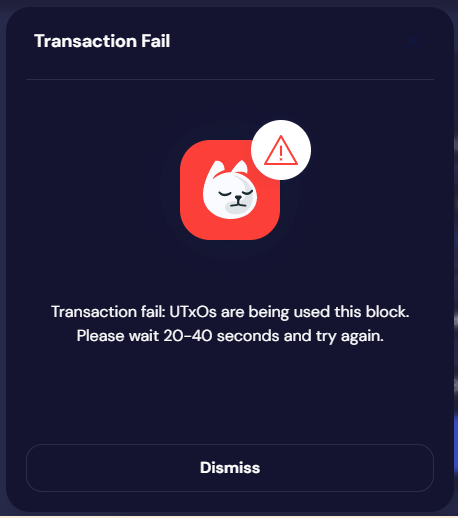
\includegraphics[scale=0.35]{minswap_errormessage}
\caption{UTXO missing..}
\end{figure}
In a blogpost \cite{minswapBlog}, Minswap appologized for the bad user experience but also argued that testnets exist to improve unfinished products: "Minswap has known about the concurrency challenge since we first began building on Cardano over 6 months ago", they wrote. "It’s an issue that every competent team and development lab building DeFi protocols on Cardano must overcome. It’s not a fundamental flaw, but is simply a design challenge that must be addressed." About a month later they published a Medium article, introducing their solution called Laminar \cite{minswapLaminar} as "an eUTXO scaling protocol for accounting-style smart contract". Sundaeswap, another project on Cardano, described the 'concurrency issue' faced by a UTXO-style DEX already earlier, in their first whitepaper \cite{sundaeswapWhitepaper} published on June 1 2021. "Because any given eUTXO can only be spent once, as part of one transaction, it appears as if only one swap can happen per block", they explained. "On the Cardano blockchain, there is roughly one block every 20 seconds. This would be abysmal throughput for a decentralized exchange."

\section{The extended UTXO model}

To understand the 'concurrency issue' it is important to understand Cardanos UTXO architecture. UTXOs are easiest explained with the cash analogy. While users of account based blockchains like Ethereum control an account whose value can be increased or decreased, users of the Cardano blockchain just control a bunch of UTXOs, all containing a certain value. As the first letter in 'UTXO' says, these outputs are 'unspent', exactly like a banknote kept in a physical wallet. And in the same way as a banknote can be spent, these UTXOs can be spent only as a whole. So, a crypto wallet holding a UTXO worth 100 Ada (Ada being Cardano's original currency) wanting to pay 20 Ada to a seller, has to put the whole amount into the transaction. The transaction will then have two outputs: a UTXO worth 20 Ada for the seller and a UTXO worth 80 Ada (minus the transaction fee, to be precise) going back to the buyer. Summarizing the result of the buy transaction: One UTXO has been spent (and will be unusable in the future) and two new UTXOs have been created (and will be usable by the the seller/buyer once the block recording the transaction is included in the ledger state). 

\begin{figure}[h]
\centering
\includegraphics[scale=0.4]{UTXO_account_model}
\caption{UTXO style vs accounting style ledger representation.}
\end{figure}

Figure 1.2 shows the difference between the UTXO and account style model: the first manipulates the ledger state through 'destruction and creation' without changing the state of variables, the second changes the ledger state through manipulation of global (account) variables. The reason why both these models exist is explained by Chakravarty et al. \cite{DBLP:conf/fc/Chakravarty0MMJ20} as follows: "Ethereum chose the account model explicitly to facilitate more expressive smart contracts. On the other hand, Bitcoin chose UTXO also for good reasons, including that its semantic model stays simple in a complex concurrent and distributed computing environment. This raises the question of whether it is possible to have expressive smart contracts, while keeping the semantic simplicity of the UTXO model." The answer given to this question by Cardano (and the authors of the above cited paper) is the eUTXO, the extended UTXO. There are four major concepts that transform a UTXO into a eUTXO:  

\begin{itemize}

\item The first extension is that the eUTXO is associated to a 'Validator' (or to be more precise: to an address given by the hash of the validator script) instead of to a public key. The validator script is a function that must evaluate to True in order to unlock UTXOs sitting at the address given by that very same validator script. Similarly in Bitcoin, scriptPubKeys are represented as BitcoinScriptAddresses with the Pay-To-Script Hash (P2SH).

\item The second change is that the eUTXO contains a 'Datum', which allows it to carry some state. To be more precise: currently, a eUTXO just contains the hash of the Datum and the spending transaction must provide the actual Datum value.   

\item The third extension is the 'Redeemer': To spend an eUTXO, this Redeemer must - as with the datum - be passed as a parameter into the validator script. The Redeemer typically describes an action. For instance if an eUTXO carries in it's Datum an exchange rate as state, a Redeemer 'update' could trigger a certain part of the validation logic in the validator. So a validator script could contain the condition that updating the state of the exchange rate is only possible for the party having created the original eUTXO while other actions like 'use' can be performed by arbitrary users.

\item The last change is that the validator script of an eUTXO sees the whole transaction that is currently being validated (a transaction can include as inputs and outputs multipe UTXOs from different script addresses and private addresses). This information, called the context, is passed into the validator as an additional argument of type ScriptContext. As the authors of the eUTXO paper explain: "The information supplied in the context enables the validator to enforce much stronger conditions than is possible with a bare UTXO model — in particular, it can inspect the outputs of the current transaction, which is essential for ensuring contract continuity." In the example mentioned in the previous point, this contract continuity would be: the eUTXO containing the exchange rate can only be spent in a transaction if a new UTXO is produced in the same transaction that also contains the exchange rate and is associated to the same script address. If this validation rule is not enforced, the exchange rate state and thus the contract continuity could get 'lost'. 
Figure 1.3 shows the most important component of the ScriptContext, the TxInfo record. It contains, as mentioned above, the list of all the outputs and all the inputs of the transaction, and also for example the amount of fees paid for the transaction (txInfoFee) or the amount of new tokens minted (txInfoImint)  

\end{itemize}
\begin{figure}[h]
\centering
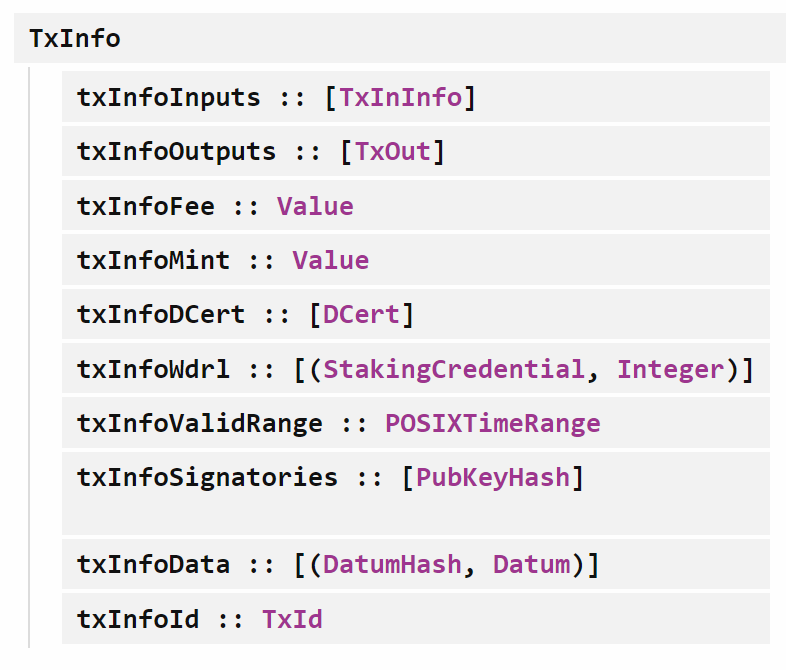
\includegraphics[scale=0.75]{context_txinfo}
\caption{Some components of the ScriptContext.}
\end{figure}
Figure 1.4 shows a Bitcoin style spending transaction, and spending UTXOs from private addresses on Cardano works this way as well. The UTXO is represented by the circle in the middle, coming as output from one transaction and going as input into a new transaction. Figure 1.5 shows the spending of a eUTXO sitting at a validator script address (again represented as the circle). For simplicity reasons I will not differentiate between UTXOs and eUTXOs from now on and just call them UTXOs.


\begin{figure}[!htb]
   \begin{minipage}{0.48\textwidth}
     \centering
     \includegraphics[width=.85\linewidth]{UTXO}
     \caption{From simple private key validation..}
   \end{minipage}\hfill
   \begin{minipage}{0.48\textwidth}
     \centering
     \includegraphics[width=.7\linewidth]{UTXO_extended}
     \caption{..to arbitrary validation logic.}
   \end{minipage}
\end{figure}

Another remark about wording in this paper: most of time, the term 'smart contract' is used to describe programs that are stored on a blockchain and run when certain conditions are met. For clarity reasons I will try to avoid it in this paper, because the term 'smart contract' is somehow misleading when it comes to Cardano (or any other UTXO style blockchain). Plutus scripts can do nothing else than returning 'True' or 'False'; they only validate transactions and never initiate an action on the blockchain on their own the way as an Ethereum smart contract can. Such an action (following a successful script evalution) must be done with off-chain code. As Cardano Founder and CEO of the development company of the blockchain Input Outuput Global (IOG) suggested, the term 'programmable validators' is therefore better suited to describe how Cardano imposes the terms of a contract.   
\begin{figure}[h]
\centering
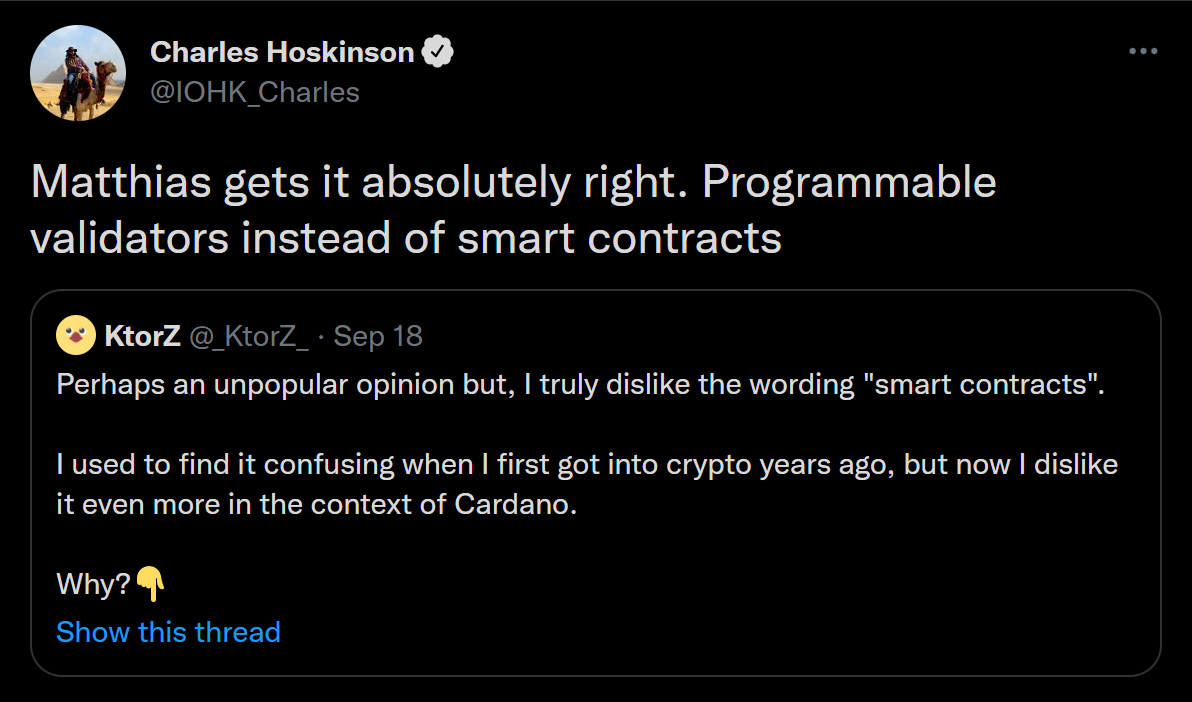
\includegraphics[scale=0.45]{programmable_validators}
\caption{No more smart contracts.}
\end{figure}

\section{The 'concurrency issue'}

Combining the fact that the state of an Ethereum style smart contract is contained in a UTXO on Cardano (e.g. the 'exchange rate UTXO' described above) and the fact that a UTXO can only be spent once brings us back to the core of the 'concurrency issue': what if two users simultaneously want to include the exchange rate contained in the UTXO in their transactions? Only one of them will get the desired input while the other user will have to try building the transaction again one block later. In this concrete case, the 'concurrency issue' is easily solved: A so-called 'oracle' that provides the exchange rate as a service can produce (and update) multiple exchange rate UTXOs for multiple users instead of just one, all containing the same exchange rate.
However if the UTXO contains as state a liquidity pool instead of an easily reproducible exchange rate, the 'concurrency issue' becomes more difficult to solve. This is the case for the DEX with automated market maker (AMM) functionality that I will describe in detail below. For now just this: An AMM-DEX UTXO contains two currencies that form a liquidity pool together. How liquidity pools work is described for example in Cryptopedia \cite{cryptopediaAMM}. One key takeaway from the article is that slippage - the percentage change in the effective price paid in a trade relative to the expected price given by the state of the liquidity pool before the trade - is a big concern in markets/pools with low liquidity. So even though in theory it is possible to split an AMM-DEX UTXO in multiple AMM-DEX UTXOs, each containing a fraction of the two currencies from the original UTXO, this is a bad idea because of increasing slippage. 

Given this contention problem over a liquidity pool, a DEX on Cardano could try to avoid having to deal with such a global state altogether and instead implement the orderbook pattern that is traditionally used by centralized exchanges. 

\paragraph{The orderbook pattern}

An order book is basically a list of open buy and sell offers for specific amounts of currency and every buy order needs to be matched with a sell order. IOG describes the order book pattern and Cardano in their docs \cite{iogOrderBook} as a natural fit: "Every order is a single UTXO, and matching a set of orders means building a transaction that spends the relevant UTXOs. The UTXOs are script UTXOs with a known address and a datum value that holds the quoted price and some bookkeeping information (for example, an address to pay the money to, and an expiration date). The currency value locked in the UTXO is the 'inverse' of the order."

While there were lots of discussions in Cardano forums about the development progress of different AMM-DEX projects, the until then little known Muesliswap DEX \cite{muesliswapDocs} went live on the mainnet at the end of November using the order book pattern. Three weeks later, it had already approached the number of 50'000 transactions with its backbone smart contract, making it the most used contract in the still short Cardano 'Alonzo' era network history.

As suggested by IOG, a UTXO paid to the Muesliswap contract contains in the Order(Datum) the name and quantity of the coin the user wants to buy (see Figure 1.7). As value, the UTXO contains the amount of the currency the user wants to sell in exchange for his buy offer. If an independent matchmaker then finds an 'inverse' offer UTXO in the ledger, he can submit a transaction with both offer UTXOs as inputs. In order for the transaction to be successful, the 'FullMatch' part of the 'mkOrderValidator' shown in Figure 1.8 must evaluate to True for both UTXOs. The central function in it being 'correctFull': It checks that the transaction contains outputs to the two public keys defined in the OrderDatum of the order UTXOs. The CancelOrder Redeemer can be triggered with only one input and comes with only one condition: only the party that has created the UTXO can spend it (i.e. transfer it back to his own wallet). This means that as long as no one else includes the order in a swap transaction with the redeemer (called OrderAction in mkOrderValidator)  'FullMatch', it can be cancelled by the owner.    

\begin{figure}[H]
\centering
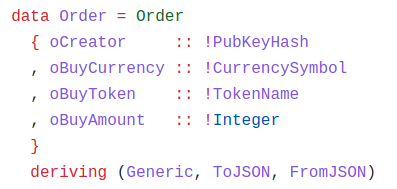
\includegraphics[scale=0.5]{muesliswap_datum}
\caption{Setting the terms for a currency exchange.}
\end{figure}

\begin{figure}[H]
\centering
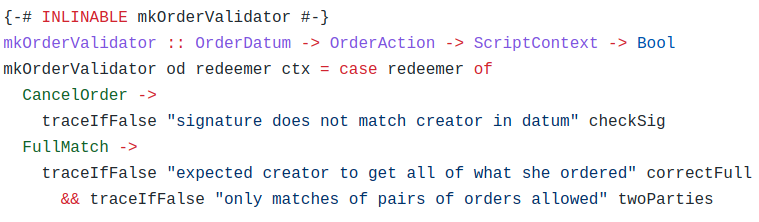
\includegraphics[scale=0.5]{muesliswap_validator}
\caption{Conditions given by the validator script.}
\end{figure} 

Also the Sundaeswap team argues, that "an order book model for an exchange, which on Ethereum is disastrously expensive to maintain and update, seems more fundamentally suited to Cardano". But they see a potential liquidity problem, meaning that no trades can be made because sell and buy offers are too far apart. "Most pools on decentralized exchanges are thinly traded", they write in a blogpost \cite{sundaeswapScalabilitySolution}: "Uniswap, for example, has over 8,000 trading pairs. If we rank the pools by trading volume and examine #30, we see only a couple of trades per hour. Consequently,we felt that a pure orderbook without the support of an AMM would be a poor fit."

\paragraph{Automated Market Maker}

Automated market makers (AMM) try to solve the problem of illiquid markets by incentivizing users to provide liquidity for a share of the trading fees. The bigger the liquidity, the less slippage will occur, as mentioned above. But even with very low liquidity, trading is always possible whereas an order book would maybe find no matches at all. Protocols like Bancor or Uniswap and basically all DEXs on account style blockchains use AMMs.

\section{Outlook}

Given the two main architectures, I decided to implement a DEX that allows concurrent swaps based on the AMM model. In the following chapters I will introduce my solution to the 'concurrency issue', which is based on a simple batching mechanism first presented by "Meld" in a Medium article \cite{meldConcurrencySolution} in mid 2021. The general idea is the following: Instead of letting the users interact directly with the contested liquidity pool state, the application allows them to make reservations. These reservations then get aggregated into one transaction involving the liquidity pool state.

In the following chapter, I will first briefly introduce an AMM DEX that doesn't address the 'concurrency issue'. Then I will show how to go from there to a concurrent DEX by introducing a reservation layer between the user and the swap transaction. In chapter 3, I will describe this reservation layer in detail, e.g by showing what conditions must be satisfied to make or to retrieve a reservation. In chapter 4 I then present the swap layer which contains the core logic of my application: It validates the swap of the aggregated reservations and makes sure that all swap participants receive the correct amount given the state of the liquidity pool. While chapters 3 and 4 describe on-chain code, in chapter 5 I introduce the importance of off-chain code for decentralized applications on Cardano. I also address the question whether applications on Cardano can be considered as truly decentralized even though they rely heavily on off-chain code.

\chapter{Dex-Design}

As (non-concurrent) basis for my project, I took the already existing application presented in a lesson of the Plutus Pioneer Program \cite{iogPlutusPioneerProgram} organized by Lars Brünjes, director of education at IOG. The app uses several Uniswap modules \cite{UniswapModules} from the Plutus library that I used as well, adjusted according to my needs and renamed as Swap modules in the src directory of my project. 

The functioning of the original DEX is summarized in Figure 2.1. Tx2 describes the creation of a liquidity pool with currencies A and B. The DEX lets an arbitrary user create such a liqudity pool - this pool technically just being a UTXO sitting at the pool script address as described above.
Bob can spend the PoolAB UTXO (resp. use it in his transaction) by fulfilling the conditions given by the PoolAB validator script. The most important part of the validation logic being that during the spending transaction (Tx3), a new UTXO must be created at the same address and that the amounts of Currency A and B contained in this new UTXO must be high enough so that their product is bigger then the product of the amounts of A and B in the old Pool UTXO.  
The validation logic follows the Uniswap protocol \cite{uniswapWhitepaper} which basically states that the product of currency A and currency B must slightly increase during a Swap, the increased value representing fees for the liquidity providers.

In this concrete example, The product A x B in the UTXO is 1'000 x 2' 000 = 2'000'000 before the execution of Tx3. After Tx3, which adds 100A to the pool and removes 181B from the pool, the product in the new UTXO is 1'100 x 1'819 = 2'000'900. So, Bob submits Tx3 with - as inputs - the PoolAB UTXO and a UTXO from his own wallet containing 100A. These 100A 'flow' into the new PoolAB UTXO which in turn allows Bob to decrease the amount of CurrencyB in the pool by 181B. Changing the amounts of currencyA and currencyB in the pool of course also affects the exchange rate offered by the DEX. Before the swap, the rate B/A is equal to 2, after the swap B/A is 1,6536.

Tx4 and Tx5 in Figure 2.1 add respectively remove liquidity from the PoolAB, Tx6 closes the liquidity pool (under the condidtion that nobody except the user executing the transaction has any liquidity left in the pool)   

\begin{figure}[h]
\centering
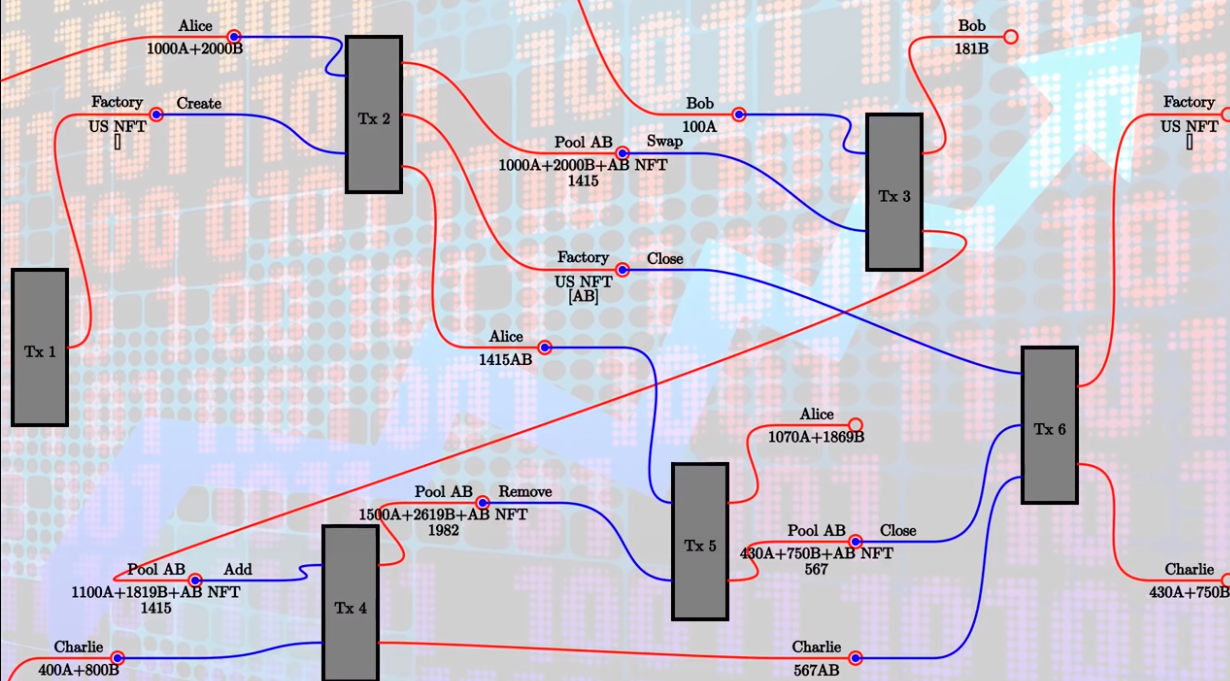
\includegraphics[scale=0.35]{Swap}
\caption{Creation (Tx2), use (Tx3), manipulation (Tx4, Tx5) and closure (Tx6) of a liquidity pool.}
\end{figure}

The 'concurrency issue' in this DEX is the fact that only one user can spend the PoolAB UTXO. Of course, the validation logic forces this user to create a new UTXO containing the updated state for the next user, but this new PoolAB UTXO is only available once the block containing Bobs transaction is added to the blockchain. This limits the DEX usage to one swap per block, with Cardano having a block interval of about 20 seconds.

\paragraph{Reserving instead of swapping} To bring concurrency into this system, an additional layer can be introduced in front of Tx3, which I will call reservation layer in this paper. Thanks to this layer, users don't interact directly with the Swap state and thus with the UTXO sitting at the address of the Pool validator script anymore. Instead, they create swap orders without touching the PoolAB UTXO. A batcher then combines these swap orders into one final transaction.
As mentioned above, this Idea was first presented by "Meld" \cite{meldConcurrencySolution}. Figure 2.2 shows these two layers, respectively transaction phases. Same as in Tx3 in Figure 2.1, the 'Apply' transaction takes as input the State (called PoolAB in Figure 2.1). But instead of just Bob's private UTXO, there are now several inputs, representing the swap orders coming out of several Reserve transactions.  

\begin{figure}[h]
\centering
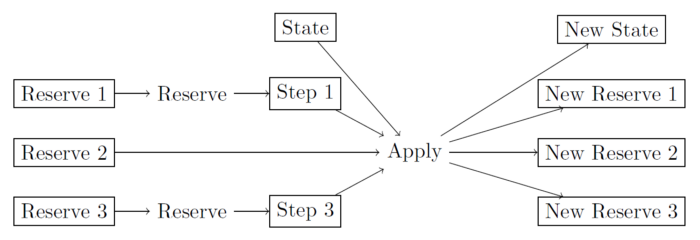
\includegraphics[scale=0.6]{meld_swap}
\caption{Including multiple swap orders into one 'Apply' transaction.}
\end{figure}

Figure 2.3 shows how these inputs are produced in earlier blocks. In Block 2, Reserve 1 is spent to create Step 1; in Block 3, Reserve 3 is spent to create Step 3; in Block 4 finally, Step 1 and Step 3 together with Reserve 2 and State from Block 1 are spent as part of the Swap transaction. The outputs of this transaction will be used as inputs for the next Swap to repeat the cycle.

\begin{figure}[h]
\centering
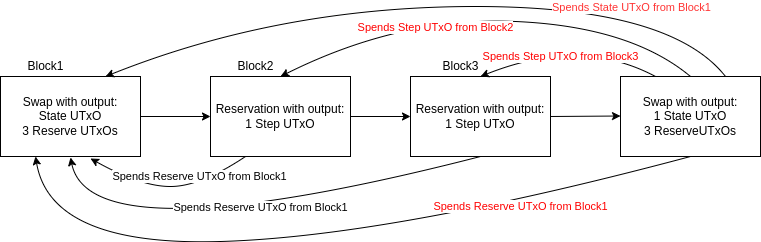
\includegraphics[scale=0.58]{Swap_inthechain}
\caption{Getting the transaction inputs from previous blocks.}
\end{figure}

In the reservation layer (left part of Figure 2.2), users can spend Reserve UTXOs and convert them into Steps (as done in Block 2 and Block 3 in Figure 2.3). In my DEX and so from now on I will call the 'Reserve' a unused reserve UTXO and the 'Step' a used reserve UTXO.

It is important to note that the batcher (i.e. the party that executes the 'Apply' transaction) cannot only include used reserve UTXOs in the transaction but must also include all the unused ones. This guarantees that no reservations are left out of the transaction and thus makes the swap deterministic. This idea was explained in the above-mentioned Medium article \cite{meldConcurrencySolution}. A weakness of this architecture however is that it leads to unnecessarily large transactions volumes if a lot of unused reserve UTXOs have to be included into swap transactions repeatedly. I addressed this problem by making the number N of Reserve UTXOs variable with a simple mechanism that I will describe later in the paper.

The 'Command' datatype below describes the command line interface of the Dex application. In my implementation, I have added the functionalities 'Reserve', 'Retrieve' and 'ReserveFunds', while the first seven commands were already available in the original IOG version (and shown in Figure 2.1). 'ReserveFunds' doesn't trigger a transaction, it only looks for used reserve UTXOs on the blockchain and reports back how many there are and the total value of currencies to swap they contain. 
'Reserve' takes as parameters two amounts (Integers) and two currencies (Chars). Executing this command will create a used reserve UTXO containing amount int1 of currency char1 and amount int2 of currency char2. Typically, one of these two amounts will be zero as it makes no sense swapping A against B and B against A at the same time. 'Retrieve' takes as arguments two currencies (chars). This command cancels a Reservation if there is a used reserve UTXO and if the transaction is initiated by the creator of the used reserve UTXO. Retrieve only cancels one reservation, so if a user made several reservations and wants to cancel all of them, he has to submit several retrieve transactions.

\begin{verbatim}
data Command =
       Funds
     | Pools
     | Create Integer Char Integer Char
     | Add Integer Char Integer Char
     | Remove Integer Char Char
     | Close Char Char
     | Swap Char Char
     | Reserve Integer Char Integer Char
     | Retrieve Char Char
     | ReserveFunds
\end{verbatim}

So basically, the first seven commands initiate actions in the Swap layer, while the last three affect the Reservation layer. I will describe the two layers in the following two chapters, starting with the Reservation layer.

\chapter{Reservation layer}

As already described above, a reserve UTXO can either be used or unused. This state is encoded in the Datum of the UTXO, called ReserveDatum. Addtionally, the Datum tells which liquidity pool the reserve UTXO is made for, how many reserve UTXOs are currently in circulation (encoded by the Integer) and - if the state is 'Used' - which public key made the reservation.

\begin{verbatim}
data ReserveDatum = Unused LiquidityPool Integer 
                    | Used LiquidityPool PubKeyHash Integer
\end{verbatim}

The Datum of the reserve UTXOs in Block 1 in Figure 2.3 is 'Unused' while the reserve UTXO produced by the transaction in Block 2 has the Datum 'Used'. Depending on the state of the Reserve UTXO, different actions are possible. These possible spending actions are checked by the reserve validator script and defined by the ReserveRedeemer:

\begin{verbatim}
data ReserveRedeemer = Reserve | Retrieve | Include | Destroy
\end{verbatim}

As the Reserve validator script below shows, a Reserve UTXO in the 'Unused' state can either be reserved, included or destroyed. A Reserve UTXO in the 'Used' state can be retrieved or included. When a new pool is created, a fixed number of Reserve UTXOs must be created in the same transaction and they are all in the 'Unused' state. After having been used and included in a swap, the state of all the Reserve UTXOs is 'Unused' again. The last two conditions are not set by the reserve validator script but by the swap validator script that I will describe in the next chapter.

\begin{verbatim}
mkReserveValidator u rs ps reserveDatum reserveRedeemer ctx =
    case reserveDatum of
        (Unused lp n) -> case reserveRedeemer of
            Reserve ->
                outputContainsFee     &&
                outputHasToken        &&
                correctLiquidityPool  &&
                correctNrReserveTokens
            Include ->
                poolStateCoinIncluded
            Destroy -> 
                uniswapIncluded &&
                outputStateUnused outputDatum
        (Used lp pkh n) -> case reserveRedeemer of
            Retrieve ->
                (Validation.txSignedBy info pkh) &&
                outputHasToken                   &&
                outputStateUnused outputDatum    &&
                correctLiquidityPool             &&
                correctNrReserveTokens
            Include ->
                poolStateCoinIncluded
\end{verbatim}

In the following paragraphs I will describe the different redeemer actions Reserve, Retrieve, Include and Destroy one by one.

\paragraph{Reserve}

To swap A against B, a user creates a used reserve UTXO containing the amount of A he wants to swap and the hash of his public key so that the party performing the swap knows to what address to pay the swapped amount of B to. This is the 'Reserve' action described in Figure 2.2. Figure 3.1 shows a transaction including a Reserve spending action in detail with all the inputs and outputs. This transaction must satisfy the conditions given by the mkReserveValidator function (code above, lines 5 to 8):

\begin{itemize}
\item outputContainsFee: The Fee in Ada must be part of the Value of the output reserve UTXO. During the swap transaction, this fee will be paid to the wallet of the user performing the swap.
\item correct liquidity pool: Because all Reserve UTXOs from all existing liquidity pools have the same Reserve Address, The lp value in the ReserveDatum associates them with the correct liquidity pool. So, to make a reservation for PoolAB, the user needs to attach a datum with the lp value 'AB'.
\item correct number of reserve tokens N: the datum also keeps track of the number of reserve UTXOs currently in circulation. By making a reservation, the user must not change this number. The number of reserve UTXOs only changes during the swap transaction: It increases if the reserve UTXOs are heavily used and decreases if the Reserve UTXOs are not much used.
\item It is maybe noteworthy that the Reserve validator doesn't force the user to create a 'Used' Reserve UTXO or to provide his public key in the ReserveDatum, as by not doing so it would be to his own disadvantage. 
\item outputHasToken: Every Reserve UTXO contains a ReserveCoin in it's value. N of these Coins are minted when the pool is created and burned when the pool is closed. Coins to identify UTXOs are very common on the Cardano blockchain. The reason is that validation only takes place when a UTXO is spent. The creation of a UTXO at a script address on the other hand comes with no restrictions. So nothing can stop a user from creating additional Reserve UTXOs for a certain pool. But having a potentially infinite number of Reserve UTXOs would make it impossible to demand that all reserve UTXOs must be included in the swap transaction in order to make it deterministic. So, instead of collecting all the Reserve UTXOs, the swap transaction collects all the Reserve UTXOs containing a ReserveCoin.
\begin{verbatim}
ownOutput :: TxOut
ownOutput = case [ o | o <- getContinuingOutputs ctx ] of
    [o] -> o
    _   -> traceError "expected only one Reserve output"

outputHasToken :: Bool
outputHasToken = isUnity (txOutValue ownOutput) rs
\end{verbatim}
The first function inspects the transaction context for outputs to the same script address as the address of the UTXO currently being validated (the reserve script address in this case). There must only be one such output, meaning that the validator doesn't allow transactions with two or more simultaneous reservations. The second function checks if the discovered output contains the above mentioned ReserveCoin (rs).  
\end{itemize}

\begin{figure}[H]
\centering
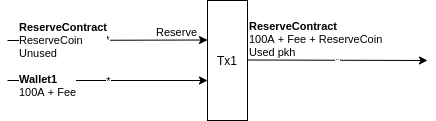
\includegraphics[scale=0.8]{reserve_def}
\caption{Creating a used reserve UTXO.}
\end{figure}

\paragraph{Retrieve}
The validation conditions for the 'Retrieve' action are much simpler: The reserve UTXO must be in the 'Used' state as it wouldn't make sense to retrieve a unused reservation. And the public key hash in the ReserveDatum must be the one from the users wallet performing the retrieve action. This guarantees that only the creator of a reservation can retrieve it. Additionally, the user is forced to create a new 'Unused' Reserve UTXO containing the ReserveCoin so that no reserve UTXOs are missing for the next Swap. 
correctLiquidityPool and correctNrReserveTokens are checked for the same reasons as in a Reserve action: The newly created unused reserve UTXO must be associated to the same liquidity pool as the old one and track the same number of reserve UTXOs in circulation.  

\begin{figure}[H]
\centering
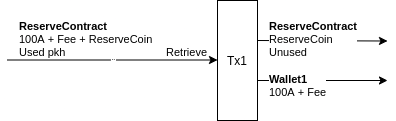
\includegraphics[scale=0.8]{retrieve_def}
\caption{Cancelling a reservation and recreating a unused reserve UTXO.}
\end{figure}

\paragraph{Include}

The most important action is obviously 'Include'. It can be performed whether the UTXO is 'Used' or 'Unused' and comes - maybe surprisingly - with only one condition: poolStateCoinIncluded. The reason for this is that the validation is delegated to the poolAB. The delegation works as follows: In the same way that a ReserveCoin identifies a Reserve UTXO, a poolStateCoin identifies a Pool UTXO. So by making sure that the poolStateCoin is part of the transaction, we also guarantee that the Pool UTXO is spent in that transaction. And the Pool UTXO can only be spent by satisfying its own validation logic (described in the following chapter). So by requiring the presence of the poolStateCoin, the Reserve validator script delegates the 'Include' validation to the Pool validator script.

This makes sense also for efficiency reasons. As IOG writes in a blog post \cite{iogDesignPattern}: 'When adopting such a batching pattern, one should bear in mind that, whenever N orders sitting at the request script are consumed within a single transaction, the request script will be executed N times on transaction submission.' Meanwhile, there is only one single state given by the poolAB UTXO, and so the Pool validator script is only executed once during the swap transaction.

\paragraph{Destroy}

The fourth and last possible action for a Reserve UTXO is 'Destroy'. This action can only be performed if the UniswapCoin is present in the same transaction. So again, this is a case of delegation of validation logic, this time by making sure that a 'PoolFactory' UTXO containing the UniswapCoin is spent in the same transaction.
Above, I used the term 'Pool validation logic' when talking about the spending of the 'Pool' UTXO while in the present context I'm talking about the spending of a 'PoolFactory' UTXO. 
Under the hood though, there is only one validator script (shown in simplified version below) for both of them. The Factory and the Pool UTXOs are UTXO instances sitting the same address, but differentiated by their Datum (either being 'Factory' with a list of liquidity pools or 'Pool' with a specific liquidity pool and an amount of liquidity coins). Because the 'PoolFactory' instance contains as value the UniswapCoin (us, passed into the validation logic in lines 8, 10 and 11 below), it can be spent with the Redeemers 'Create' or 'Close' as shown in the simplified code below. For a UTXO not containing this coin, validateCreate, validateCloseFactory and validateClosePool would not validate. 

\begin{verbatim}
mkUniswapValidator :: Uniswap
                      -> UniswapDatum
                      -> UniswapAction
                      -> ScriptContext
                      -> Bool
mkUniswapValidator us Factory Create = validateCreate us
mkUniswapValidator _  Pool    Swap   = validateSwap 
mkUniswapValidator us Factory Close  = validateCloseFactory us
mkUniswapValidator us Pool    Close  = validateClosePool us
mkUniswapValidator _  Pool    Remove = validateRemove
mkUniswapValidator _  Pool    Add    = validateAdd
mkUniswapValidator _  _       _      = False
\end{verbatim}

So, coming back to the Reserve UTXOs: given the delegation of validation, they can and must be destroyed - respectively their ReserveCoins must be burned - when a Pool is closed and so this condition is included in the 'validateClosePool' function. Burning the coins is important, because otherwise lingering ReserveCoins would exist that could be used to create additional valid Reserve UTXOs. A second condition for destroying reserve UTXOs, also given by the mkUniswapValidator, is that the state of the reserve UTXOs being 'destroyed' must be unused. otherwise, the user that made the reservations would loose his money.

\chapter{Swap layer}

\paragraph{Swap} After having described the reservation layer, I'm coming now to the second layer, in which the 'Apply' transaction from Figure 2.2 takes place. As already mentioned, the (used and unused) reserve UTXOs must be included in this transaction with the redeemer 'Include'. And as also mentioned, the validation logic is delegated to the spending of the pool UTXO through the 'poolStateCoinIncluded' function. Figure 4.1 shows all the inputs and outputs of this transaction.

\begin{figure}[h]
\centering
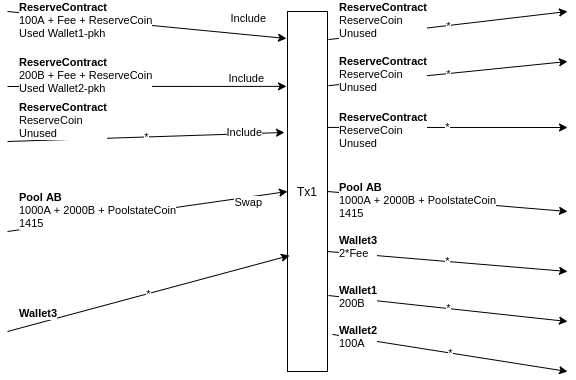
\includegraphics[scale=0.6]{swapWithoutSwapContract}
\caption{Swapping the orders made by Wallet1 and Wallet2.}
\end{figure} 

As Figure 4.1 shows, the Pool UTXO is spent with the 'Swap' redeemer. This triggers the 'validateSwap' function, the ninth line of the mkUniswapValidator script above shown here in more detail: 

\begin{verbatim}
mkUniswapValidator _  c r (Pool lp _) Swap ctx = validateSwap r lp c ctx
\end{verbatim}

To evaluate to True, validateSwap must fulfill the following conditions:

\begin{verbatim}
    allClientsReceiveCoins        &&
    allReserveOutputsPresent      &&
    allReserveInputsPresent       &&
    checkSwap oldA oldB newA newB &&
    (isUnity inVal c)             &&
    (isUnity outVal c)            &&
    noUniswapMinting
\end{verbatim}
\begin{itemize}
\item allReserveInputsPresent: This condition makes sure that all the reservations - whether they are 'Used' or 'Unused' - are included in the swap transaction. The function gets the correct amount of reserve UTXOs from the Datum of any of the reserve UTXOs.

\item allReserveOutputsPresent: Part of the swap validation is a mechanism to determine the number N of Reserve UTXOs for the next reservation round. This is done by looking at the ratio r of the used number to the total number of reserve UTXOs. If r is above 0.7, an additional ReserveCoin is minted and included (in an additional Reserve UTXO) in the transaction output. If the ratio is below 0.3 and there are more then 3 reserve UTXOs in the transaction input, a ReserveCoin is burned. The allReserveOutputsPresent function checks that the transaction output contains exactly the new number of reserve UTXOs (nrNewRes).

\begin{verbatim}
nrNewRes
    | nrUsedRes/nrOldRes >= .7 = nrOldRes + 1
    | nrUsedRes/nrOldRes <= .3 = max 3 (nrOldRes - 1)
    | otherwise             = nrOldRes 
\end{verbatim}

This is a very simple way of adjusting the number of reserve UTXOs. It could of course be done in a more sophisticated way by determining the newNrReserveTokens based on the information of multiple previous rounds instead of just one. 

\item allClientsReceiveCoins: This is really the core function of my whole program. It makes sure that everyone that made a reservations will receive the correct amount out of the swap transaction. 
To validate, the following function must evaluate to True:
\begin{verbatim}
allClientsReceiveCoins = valuesToPay == valuesPaid
\end{verbatim}

'valuesPaid' is a list of all the payments to all the PublicKeys observed in the transaction. It is easy to get thanks to the ScriptContext parameter that contains this information. 

'valuesToPay' is more difficult to construct. The goal for this function is to be deterministic (meaning that given a set of inputs, it always delivers the same output), so that the party building the swap transaction cannot manipulate it. A manipulation could be done for example by first applying all the sell reservations of currencyA to the liquidity pool and thus increasing the relative amount of currencyA in the pool (resp. lowering the relative value of currencyA). Then, the swap executor could first apply his own reservation for buying A before all the others, thus getting currencyA for lower price.

Meld suggests in the above mentioned  article \cite{meldConcurrencySolution} applying timestamps to the reservations and then applying them to the liquidity pool in the order given by these timestamps.

In my implementation though, the reservations are not applied to the liquidity pool one by one. Instead, the first step is to calculate the difference of the total inputs of currenies A and B, 'SwapInputAmountA x r - SwapInputAmountB'. r is the ratio of 'totalAmountB / totalAmountA' in the liquidity pool before the transaction and thus the current exchange rate. And so 'SwapInputAmountA x r' is the value of the input of CurrencyA expressed in terms of CurrencyB. 
The second step is to apply 'SwapInputAmountA x r - SwapInputAmountB' to the liquidity pool if the difference is positive (meaning that the value of all CurrencyA inputs is bigger then the value of all CurrencyB inputs). Otherwise, 'SwapInputAmountB - SwapInputAmountA x r' is applied.

The following function returns this amount, the second amount being equal to zero in each case. 
\begin{verbatim}
amountForSwapInput :: Integer -> (A, B) -> (A, B)
amountForSwapInput r (a,b)
    | a * r > b = (a - b / r, 0)
    | otherwise = (0, b - a * r)
\end{verbatim}

So only either CurrencyA or CurrencyB is applied to the liquidity pool (or neither, in case of TotalCurrencyA * r = TotalCurrencyB). If CurrencyA is applied, that means that the total value of all the CurrencyA inputs (in terms of CurrencyB) is bigger then the total value of all the CurrencyB inputs. So the users that made reservations to sell CurrencyA will get all the CurrencyB inputs plus the result of the swap. The users that made reservations to sell CurrencyB just get the amount TotalCurrencyB / r from the TotalCurrencyA input.

The result of this logic are the following functions: 

\begin{verbatim}
totalValA' :: Amount A
totalValA'
    | newA - oldA > 0 = totalValB / r
    | otherwise       = (oldA - newA) + totalValA 

totalValB' :: Amount B
totalValB'
    | newA - oldA > 0 = (oldB - newB) + totalValB
    | otherwise       = totalValA * r 
\end{verbatim}

totalValA' is the amount that will be distributed between the users swapping CurrencyB for CurrencyA and totalValB' is the amount that will be distributed between the users swapping CurrencyA for CurrencyB. oldA, newA, oldB and newB are the values in the liquidity pool before and after the swap. 

        In the transaction shown in Figure 4.1, 'totalValA * r' is equal to 'totalValB' (the exchange rate r, given by 1000A and 2000B, is 2, so the 100 A are worth 200 B). This means that the inputs can be swapped directly. The suppliers (in this case only one, wallet1) of the 100 A get the 200 B and the suppliers of the 200 B (wallet2) get the 100 A. The PoolAB UTXO must of course be included in the transaction anyway as it provides the exchange rate r and as Reserve UTXOs can only be spent in the presence of a PoolStateCoin.

Once the total amount of A and B in the output is known, it must be made sure that the providers of CurrencyA get the correct share of the output of CurrencyB and vice versa. This is done by calculating the percentage of the total input of one currency provided by a user and guaranteeing that he gets the same percentage of the output of the other currency.

For example: If User1 supplies 10 percent of the total input of currencyB, he must get 10 percent of the total output of currencyA.

One problem with this implementation was that the equality condition 'valuesToPay == valuesPaid' doesn't hold if the party performing the Swap transaction himself also made reservations. This is because the value paid to the public key of the party performing the swap includes the fees paid by the other users. To solve the problem, reservations from a public key performing the swap are filterd out before the 'allClientsReceiveCoins' function is run.

The logic behind this is the following: The validator guarantees certain conditions for all third party users paying money to the script address. Once these conditions are satisfied by a transaction and there is still money left to spend, this 'excess' amount goes automatically to the wallet of the party submitting the transaction. In the case of the swap transaction this means that once every user gets a UTXO with the percentage of the output he is entitled to, to party performing the swap can take all the rest (thus including the fees). If he doesn't agree with this output, he simply doesn't submit the transaction.

\item The four remaining conditions (checkSwap, isUnity inVal c, isUnity outVal c and noUniswapMinting) were given by the original Uniswap script, with checkSwap being the implementation of the above mentioned UniswapV1 protocol. The values for the arguments oldA and oldB are coming from the Uniswap UTXO being spent in the transaction and the values of newA and newB from the Uniswap UTXO being created in the transaction. Getting the amountForSwapInput for one currency (the other being zero) from the function described on page 16, the app calculates how much of the second currency it can take out of the liquidity pool without invalidating the checkSwap function.  
\end{itemize}

\paragraph{Create/Close}
As already mentioned, the transaction creating a Pool UTXO must also create the correct amount of Reserve UTXOs. For simplicity reasons, I have hardcoded this number to three in the validator script:
\begin{verbatim}
amountOf minted r == 3    
\end{verbatim}
The number of ReserveCoins that must be burned when a pool is closed cannot not be hardcoded because it gets adjusted during every swap transaction in its lifespan. The final number of ReserveCoins is encoded in the Datum of every reserve UTXO and can be retrieved easily: 
\begin{verbatim}
amountOf minted r == negate nrReserveTokens    
\end{verbatim}

The remaining redeemer actions Remove and Add, invoked to add/remove liquidity to/from a pool are not impacted by my implementation and so I will not describe them here.

\chapter{On-chain and off-chain components}
A potential flaw making my DEX completely unusable would be to not set a maximum amount for the reservations. I describe this problem in detail because it illustrates very well potential limitations coming with the fact that script validation takes place in the narrow transaction context (ScriptContext). The problem is the following: If the total amount of a currency locked in the reserve UTXOs is bigger then the amount of that currency in the liquidity pool, the swap cannot happen because the amount of a currency in a liquidity pool must never become negative (nor zero, as the product of the two currencies must increase with every swap). At the same time, the swap validator doesn't allow the swap transaction to leave aside any reservations as the inclusion of all the reservations is mandatory to make the swap deterministic. So unless enough reserve UTXOs get cancelled by the users or the amount of the currency in the liquidity pool increases, the swap transaction can never happen.

The easiest solution for this problem would be to just limit the amounts of currencyA and currencyB a user can put into a reserve UTXO to the amounts of
\begin{verbatim}
oldA/nrReserveTokens
oldB/nrReserveTokens
\end{verbatim}
respectively, where oldA and oldB are the amounts of A and B in the pool before the swap. Given these conditions, all reservations together could never exceed the amount contained of the liquidity pool of either currency. But: The PoolAB UTXO that holds the information about oldA and oldB is not included in the reserve transaction. So, because the validator only sees the scriptContext and not the whole ledger, the conditions cannot be checked. Including the PoolAB UTXO is of course no option - as not needing it for every reservation is what made this DEX concurrent in the first place. 

The problem can be solved, though, with minimal on-chain computation. Instead of checking the conditions in the reservation layer, all my DEX implementation does is filter out the used reserve UTXOs (each containing amtA of currencyA and amtB of currencyB) during the swap validation with the following lambda function:
\begin{verbatim}
(amtA, amtB) -> amtA <= oldA/nrReserveTokens && 
                amtB <= oldB/nrReserveTokens
\end{verbatim}
The idea behind this is that the swap validator guarantees the correct output if the user follows the rule of not reserving more than 'oldA/nrReserveTokens' of currencyA and 'oldB/nrReserveTokens' of currencyB. Making sure that this doesn't happen, meanwhile, is the job of the off-chain code that I haven't described yet. 

The off-chain part of a Plutus application is code written in Haskell (while the On-chain part is written in Plutus, a subset of Haskell, and pre-compiled to Plutus core by the GHC plug-in called Plutus Tx). The job of the off-chain code is basically to build transactions that can be submitted to the blockchain and making sure that these transactions will pass the validation logic. The transaction building, of course, can be done with the 'outside' knowledge of the whole ledger state. So it is easy to check the following conditions before submitting the transaction to the blockchain and abort the process by throwing an error if the conditions are not met:
\begin{verbatim}
when (amountA >= poolAmtA/nrReserveTokens) || 
     (amountB >= poolAmtB/nrReserveTokens) 
      $ throwError "reservation exceeds limit"
\end{verbatim}
the values of amountA and amountB to be swapped are coming from the uniswap-client (in the app directory of my project), which constructs for the user the cli described on page 9. The uniswap-client submits the command entered by the users via http-request to the uniswap-pab, which is the server component of the Uniswap app. The 'pab' in uniswap-pab stands for Plutus Application Backend \cite{iogPAB} and it is - among other things - used to forward user input to the running contract instances defined in the off-chain code. My program submits the transactions defined in the contracts to a simulated blockchain initiated by the Plutus.PAB.Simulator module \cite{iogPabSimulation}

The on-chain swap validator script filtering out reservations that exceed a certain amount could be more sophisticated. For example, it could guarantee that users that made reservations exceeding the limit get their money back during the swap transaction. This would come with the advantage of users non having to make sure that the off-chain code (which can be provided by different implementations for the same on-chain code) aborts transactions with reservations that are too big. The disadvantage on the other hand is that there is more on-chain computation which of course is much more expensive then off-chain computation.

\paragraph{Decentralized or not?}
The example above shows very well the different degrees of decentralization of Cardano apps. One could argue that they are not decentralized at all, since the on-chain part is just a programmable validator that validates transactions and never jumps into action otherwise - so there can be no smart contract that waits for reservations and then, once the are part of the ledger, performs the aggregated swap by itself. But a well written validator guarantees that exactly the intended (and only the intended) swap can be performed by some off-chain code. 

If these guarantees are properly encoded in the validator script, users don't need to trust the party performing the swap. That's why Sundaeswap, when comparing different architectures for DEX implementations on Cardano, gave all of them high scores in the category decentralisation (see Figure 5.1). The only model that doesn't get the highest decentralization score, 'Governed Scoopers' is the one they decided to implement. As they explain in a Medium article \cite{sundaeswapScooperModel}, they first leaned towards the 'Escrow Tokens' model, which is the one I implemented for this thesis. "Unfortunately", they note, "this solution crashes head first into the sizing limits of the Cardano blockchain", explaining that "in practice, our first implementation of this was hitting the Cardano protocol limits with 5 or 6 escrow tokens, before even adding in features like governance."

\begin{figure}[h]
\centering
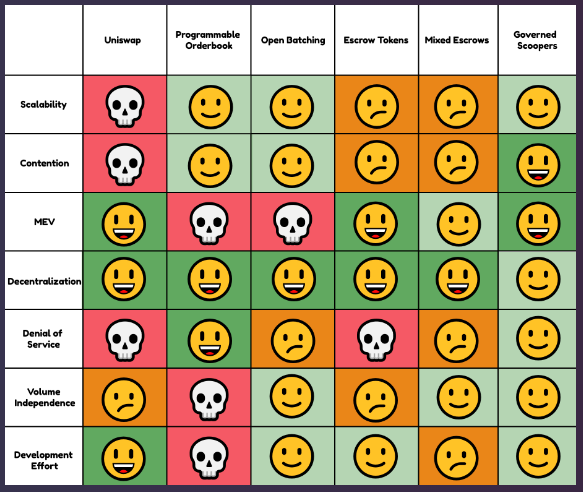
\includegraphics[scale=0.6]{comparison_sundaeswap}
\caption{Scores given to different DEX architectures by Sundaeswap \cite{sundaeswapScooperModel}.}
\end{figure} 

They decided to sacrifice a little bit of decentralization for better scores in other categories. "If you can trust your aggregators to consistently and fairly choose which orders to include, you no longer need escrow tokens, for example. You can focus on that contention-less on-ramp, and on protocol composability", they explain. SundaeSwap will try to establish a "limited amount of trust in the aggregators" by, as one of the mechanisms, licensing them and giving the SundaeSwap community the power to revoke these licences via a vote.

\chapter{Conclusion}

\paragraph{Further development} The Sundaeswap arguments in the previous chapter show that my DEX implementation is hardly usable as a real world application (in addition to the fact that I didn't use the newest version of the Plutus language and the PAB as these components were still evolving when I started writing this thesis), but it demonstrates how the problem of a single state being under a lot of contention can be solved by introducing an additional layer. This pattern will - in combination with other techniques - surely be used in some AMM-style DEXs appearing on the Cardano blockchain in the coming months.

A quite radical way to avoid triggering the N reserve validator scripts that come with the additional reserve layer while still having the same degree of concurrency was presented in September by IOG in the already mentioned blogpost \cite{iogDesignPattern}. The idea is that users only send a notification to the reservation layer and the order itself to their own public key address. All order UTXOs sitting at wallet addresses must contain an 'order’ token so that the batcher can identify them and build the aggregated swap transaction. Because the orders are sitting at public key addresses, no validator script has to be run to spend them (the notifications in the reservation layer are only inspected to find the orders, but not spent). This pattern comes with the disadvantage though that all users must be online to sign the aggregated transaction to authorize the spending of their orders. 

Additionally, IOG is developing hydra heads \cite{iogHydra} as an isomorphic layer 2 solution where DEXs could build their swap transactions in the future. This would solve the problem of the transaction size limit that stopped Sundaeswap from further developing their 'Escrow Tokens' model.

\paragraph{Worth the trouble?} Given the difficulties of building a concurrent AMM style DEX on Cardano: Is the UTXO model worth it? My personal opinion is of course of little relevance, especially as I have no experience building DEXs on account-style blockchains. But still, a number of strong arguments in favour of the UTXO model seem obvious to me. First and most importantly: In contrast to f.ex Ethereum, on the Cardano blockchain a correctly built transaction can never fail in mid-script execution. As IOG explains \cite{cardanoEUTXOExplainer}, "the success or failure of transaction validation depends only on the transaction itself and its inputs, and not on anything else on the blockchain. As a consequence, the validity of a transaction can be checked off-chain, before the transaction is sent to the blockchain." This means that a transaction only fails if some other transaction concurrently consumes an input that the transaction is expecting - or if the off-chain code is badly written and the transaction is submitted anyway. The first scenario is checked in the phase-1 validation and the second scenario in phase-2 validation \cite{cardanoCollateral}. To discourage denial of service attacks through submitting faulty transactions and to guarantee that the validator nodes are compensated for their work in case phase-2 validation fails, a collateral is used. But if already phase-1 validation fails (because the on-chain conditions have changed since the transaction was constructed), the transaction is rejected entirely without any fees or collateral being charged.
Another argument for the UTXO model is that the fees for a valid transaction are deterministic because given the same inputs, the validation always produces the same result as the global ledger state does not influence it. This means that transactions on Cardano are not in danger of 'running out of gas' as Ethereum smart contract executions are.

As a last point: Developers might have to find innovative solutions to make their apps concurrent due to the 'local' nature of transaction validation. But the other side of the medal is that this 'local' nature of transaction validation makes a high degree of parallelism possible. "A node could, in principle, validate transactions in parallel, if those transactions do not try to consume the same input", so the above mentioned explainer \cite{cardanoEUTXOExplainer}. "This is great both for efficiency and for reasoning, simplifying the analysis of possible outcomes, and proving that ‘nothing bad’ can happen."

\bibliographystyle{ieeetr}

\bibliography{references}

% mandatory declaration of origin, this must be the last page
\chapter*{Erklärung}

\emph{Erklärung gemäss Art.~30 RSL Phil.-nat. 18}

\vspace*{1cm}

\noindent
Ich erkläre hiermit, dass ich diese Arbeit selbstständig verfasst und keine
anderen als die angegebenen Quellen benutzt habe. Alle Stellen, die
wörtlich oder sinngemäss aus Quellen entnommen wurden, habe ich als solche
gekennzeichnet. Mir ist bekannt, dass andernfalls der Senat gemäss Artikel
36 Absatz 1 Buchstabe r des Gesetzes vom 5. September 1996 über die
Universität zum Entzug des auf Grund dieser Arbeit verliehenen Titels
berechtigt ist.

\vspace*{1cm}

\noindent
Für die Zwecke der Begutachtung und der Überprüfung der Einhaltung der
Selbständigkeitserklärung bzw.  der Reglemente betreffend Plagiate erteile
ich der Universität Bern das Recht, die dazu erforderlichen Personendaten
zu bearbeiten und Nutzungshandlungen vorzunehmen, insbesondere die
schriftliche Arbeit zu vervielfältigen und dauerhaft in einer Datenbank zu
speichern sowie diese zur Überprüfung von Arbeiten Dritter zu verwenden
oder hierzu zur Verfügung zu stellen.

\vspace*{5cm}

\par\noindent\makebox[6cm]{\hrulefill}   \hfill\makebox[8cm]{\hrulefill}
\par\noindent\makebox[6cm][l]{Ort/Datum} \hfill\makebox[8cm][l]{Unterschrift}

\end{document}
